\documentclass[12pt, a4paper]{article}

% for Chinese
\usepackage{fontspec}               		% 加這個就可以設定字體
\usepackage[BoldFont, SlantFont]{xeCJK} 	% 讓中英文字體分開設置
\setCJKmainfont{新細明體}            			% 設定中文為系統上的字型,而英文不去更動,使用原TeX\字型

% useful packages
\usepackage{amsfonts}
\usepackage{amssymb}
\usepackage{amsmath}
\usepackage{amsthm}
\usepackage{epsfig}
\usepackage{graphicx}
\usepackage{natbib}
\usepackage{textcomp}
\usepackage{booktabs}
\usepackage{multirow}
\usepackage{fullpage}

% some basic setting
\parskip=5pt
\footnotesep=5mm
%\lineskip=10pt
\parindent=24pt % 為了讓中文文章的首句縮排是空兩格
\renewcommand{\baselinestretch}{1.2} % 中文文件 1.2 以上較佳

% theorems, lemmas, argmin, argmax, etc.
\newtheorem{lemma}{Lemma}
\newtheorem{ques}{Question}
\newtheorem{prop}{Proposition}
\newtheorem{defn}{Definition}
\newtheorem{rmk}{Remark}
\newtheorem{note}{Note}
\newtheorem{eg}{Example}
\newtheorem{aspt}{Assumption}
\DeclareMathOperator*{\argmax}{argmax}
\DeclareMathOperator*{\argmin}{argmin}

% "摘要", "表", "圖", "參考文獻"
\renewcommand{\abstractname}{\bf 摘要}
\renewcommand{\tablename}{表}
\renewcommand{\figurename}{圖}
\renewcommand{\refname}{\bf 參考文獻}



% title information
\title{\LaTeX 入門}
\author{孔令傑\thanks{國立臺灣大學資訊管理學系副教授;lckung@ntu.edu.tw。
	版權沒有,歡迎分享;如果發現錯誤,請跟我說。}}
\date{2020 年 7 月 3 日} 

\begin{document}
\maketitle

%\fontsize{20}{20pt}\selectfont





\begin{abstract}
\hspace{1pt} 這是一個簡單又陽春的 \LaTeX 入門教學,寫給我的學生看的。
我們介紹基本的安裝與編譯,以及一些最基本的功能。本文中也提到一些延伸閱讀,
供有興趣的同學深入學習。
\end{abstract}










這是一個簡單又陽春的 \LaTeX 入門教學,寫給我的學生看的。
我始終相信要令人相信一篇文章有內涵,必要條件是在寫作上下功夫,
而這至少包含對作文能力的鍛鍊與對排版的要求。退一萬步講,好好排版是一個作者的責任,
而這正是使用 \LaTeX 的最大原因。

本文除了介紹一些基本觀念與指令,也描述一些我個人在寫作與排版上的習慣和要求。
希望各位的同學能盡量配合,最好連原始碼也用跟我類似的方式寫,以節省大家的時間。











\section{安裝與編譯}

安裝一般泛稱為 \LaTeX 的文字編輯系統,並且讓它支援中文,在現在這個時代已經非常容易了。
基本上建議你要下載並安裝的是名為 MikTeX 的系統\footnote{http://miktex.org/。},
在此刻的版本是 2.9.7442(截至2020.7.3)。你可以把 MikTeX 想成是一個編譯器(compiler),
它會把你將來寫的 \LaTeX \ source code 編譯排版成文稿。
想當然爾,如果有一個好的編輯器(editor),會讓你事半功倍。在此刻,
我用的是 Texmaker 這個編輯器\footnote{http://www.xm1math.net/texmaker/。},
我個人十分推薦。你如果想用其它的編輯器,當然也可以,有操作的問題不要問我就是了。
一個很多人用的編輯器是 WinEdt,但它不是免費的,我當然也不希望你盜版。
這兩個軟體都是下載安裝檔後一直按下一步就可以安裝完了,過程中如果有些小問題,
看一下 manual 或上網查一下也可以輕易解決,我就不贅述了。

我們寫出來的 source code 會被存在附檔名為 TEX 的原始檔中。一般我會用下列三種方法做編譯:
\begin{enumerate}
\item 純英文、非投稿到期刊\footnote{只有這個方案下可以讓 Texmaker 內建的 PDF 瀏覽器與 TEX 編輯區連結。
		這很方便!}:
		用 PDFLaTeX 直接編譯成 PDF 檔。
		文稿中的圖形必須是 JPEG、PNG 等一般點陣圖格式。
		在 Texmaker 裡,我會把 PDFLaTeX 和瀏覽 PDF 這兩個動作一起設定為由 F1 觸發。
\item 純英文、投稿到期刊:用 LaTeX 編譯出 DVI 檔、用 Dvipdfm 產生 PDF 檔,
		再瀏覽 PDF。文稿中的圖形必須是 EPS 這種向量圖。
		在 Texmaker 裡,依序是按 F2、F9 與 F7。
\item 有中文:將上方列的編譯方式改為 xeLaTeX ,編譯出 PDF 檔,再瀏覽 PDF。圖片格式跟 PDFLaTeX 支援的一樣。
		此時必須要在 TEX 檔的最前面加入本說明文件最前面那幾行 code,並且將 TEX 以 UTF-8 格式儲存,
		才能正確支援中文。我會手動把 Texmaker 裡的 LaTeX 改成 xeLaTeX,
		然後依序以 F2 和 F7 執行。
\end{enumerate}

打開「選項」中的「設定 Texmaker」,可以簡單地設定上述的三種編譯方法。
若不使用快速鍵,則需按下上方列的「XeLaTex」左邊的箭頭來重新編譯,再按下「瀏覽PDF」左邊的箭頭來更新畫面。
圖 \ref{fig:compile1} 的設定是給 xeLaTeX 用的,上方紅框建議改成圖中顯示的那樣
(在最前面加上 xe)\footnote{xeLaTeX 已經內建於現在的 MikTeX 了。
關於其詳細設定與使用方法,請上網以 xeLaTeX 和 Texmaker 做關鍵字搜尋。};
下方的紅框則是讓你設定使用 Texmaker 內建的 PDF 瀏覽器,這樣瀏覽器才能與 TEX 編輯區連結。
圖 \ref{fig:compile1} 的設定是把 F1(快速編譯)設定成 PDFLaTeX 和瀏覽 PDF。

		\begin{figure}
		\centering
		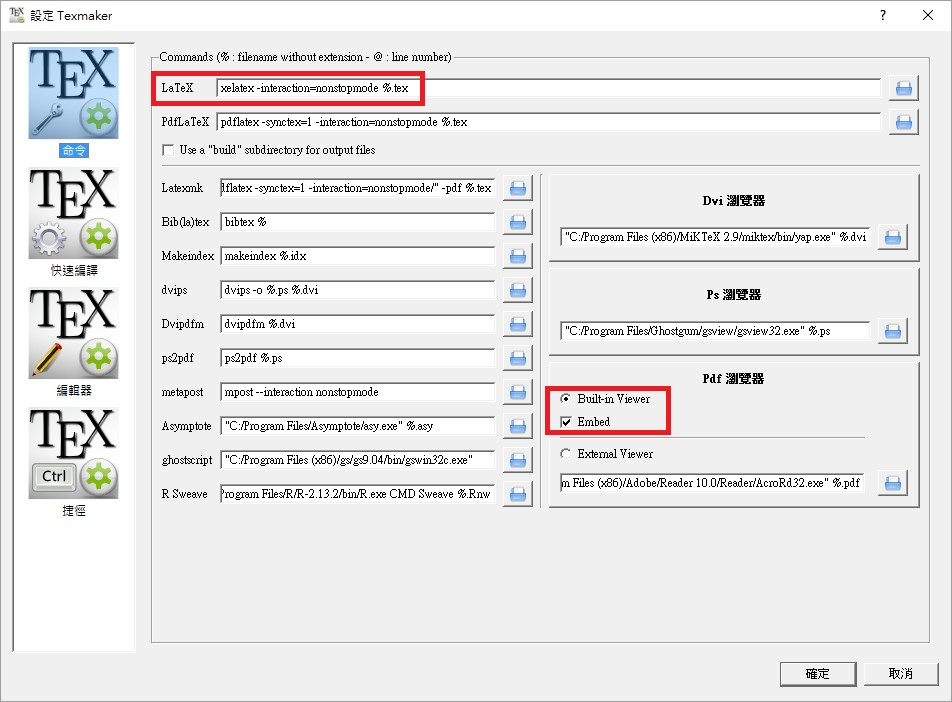
\includegraphics[width=0.8\textwidth]{figures/compile1}
		\caption{使用 xeLaTeX}
		\label{fig:compile1}
		\end{figure}

		\begin{figure}
		\centering
		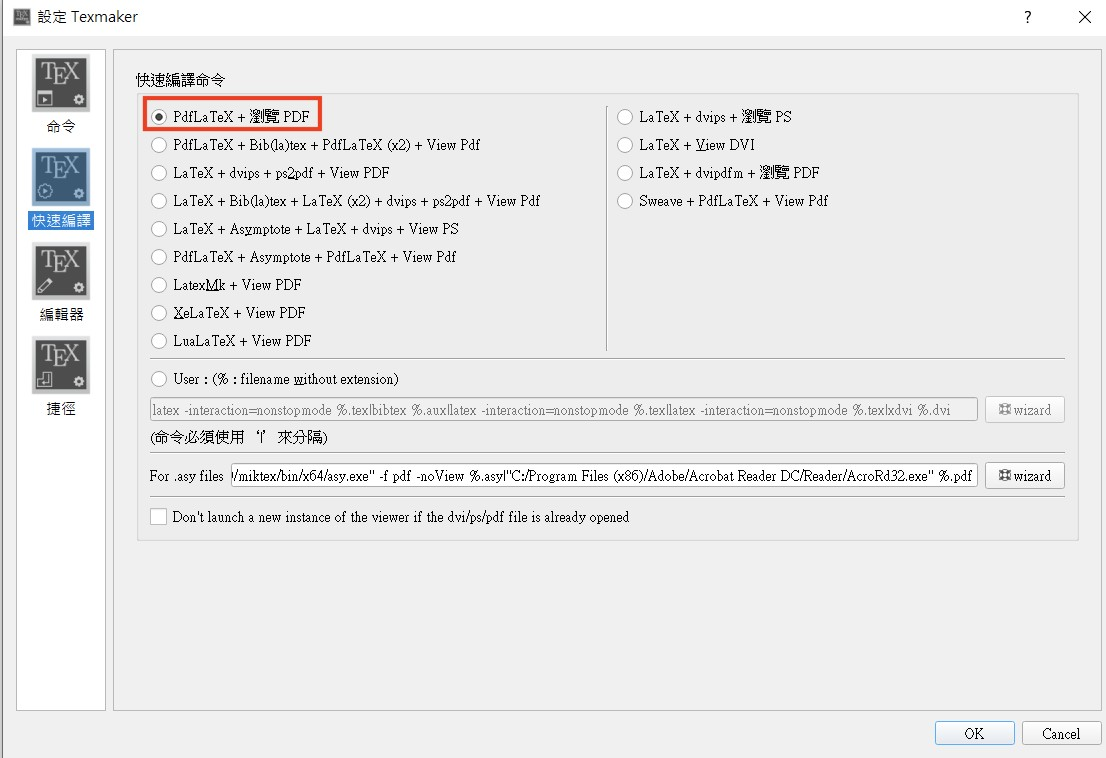
\includegraphics[width=0.8\textwidth]{figures/compile2}
		\caption{使用 PDFLaTeX 並瀏覽 PDF}
		\label{fig:compile2}
		\end{figure}

網路上有許多 \LaTeX 的相關資源,
其中「cwTeX3 手冊」是一本不錯的入門書\footnote{http://homepage.ntu.edu.tw/\textasciitilde ntut019/cwtex/cwtex.html。},
雖然其中很多關於中文的部份已經不需要了(cwTeX 在沒有 xeLaTeX 前是最普遍的 LaTeX 中文套件),
但許多關於排版的知識以及 \LaTeX 的語法介紹還是非常值得一讀。PTT 上也有 LaTeX 板,大家可以多加利用。
以下我為一些最最基本的功能提供範例。



















\section{章節}

在一篇文章中,我們用 \verb|section| 標示「節」,用 \verb|subsection| 標示「小節」,
要是還不夠,可以用 \verb|subsubsection| 來製造「小小節」。
你可以看到,只要用 \LaTeX 預設的版面,不多做設定,看起來就蠻正式的了。










\section{方程式}

在 \LaTeX 中寫數學式很容易,用兩個「\verb|$|」把數學式子框起來即可,
像是 $\alpha + \beta_2 + \frac{\gamma}{\ln \xi}$。像這樣放在文章中的式子,
我們叫它「隨文數式」。當方程式很長或需要被強調時,我們將方程式獨立成行,
寫成「展示數式」,像是這個 regression model
\begin{equation}\label{eq:reg}
	y = \beta_0 + \beta_1 x_1 + \beta_2 x_2
\end{equation}
就是一個常見的例子。使用 \verb|equation| 環境時,方程式會自動編號,
如果用 \verb|\[ \]| 環境,像是
\[
	F = ma\mbox{,} 
\]
就不會了。

有時候方程式需要換行,像是
\[\begin{split}
	y &= 3 + 5 \times 2 \\
		&= 3 + 10
\end{split}\]
這樣,或甚至像這個 LP(Linear Program):
\begin{equation}\label{eq:LP}\begin{split}
	\max \quad & x_1 + x_2 \\
	\mbox{s.t.} \quad 
	& x_1 + x_2 \leq 6 \\
	& x_1 + x_2 \geq 6 \\
	& x_1 \geq 0 \mbox{、} x_2 \geq 0\mbox{。} 
\end{split}\end{equation}
請特別注意即使是展示數式,只要方程式的結尾是句子的結尾,就應該要有標點符號。
因為本篇文章是中文文章,所以要用中文標點,
而方程式環境中不能直接顯示中文符號,所以要用 \verb|mbox| 包起來,
寫中文文章時請多留心。

大家常常會寫到最佳化問題,請注意它對齊的方式:$\max$ 跟 s.t. 靠右對齊,
其它式子則靠左對齊。換行有很多種作法,當只有一個地方要對齊,我喜歡用 \verb|split|,
因為它會把方程式編號垂直置中,像 (\ref{eq:LP}) 這樣。
當有兩個地方要對齊,我會用 \verb|eqnarray| 或 \verb|array|;三個以上,
就會用 \verb|array| 了。另一個很常用的環境是 \verb|align|,常搭配 \verb|notag| 使用,
大家可以去查查看。













\section{圖與表}

\subsection{圖}

你可以如圖 \ref{fig:res1} 那樣插入一張圖(我喜歡把圖片放在名叫「figures」的資料夾裡),
也可以把兩張圖併排,像圖 \ref{fig:res1again} 跟 \ref{fig:res2} 那樣。
請注意中文文件應該寫「圖 1」而非「Figure 1」,這個我們在這個範例檔的最前面有設定,
你看一下就知道怎麼設定了。插入圖片(或表格)時可以設定其位置(範例檔中的 \verb|[hbt]|),
你可以查查看怎麼用;不然就用預設的,通常效果也夠好了。

\begin{figure}[hbt]
\centering
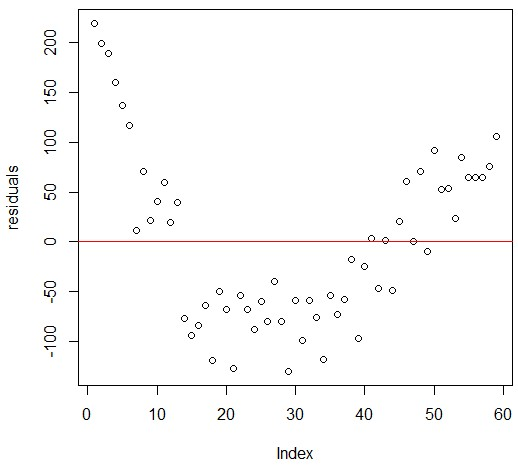
\includegraphics[width=0.4\textwidth]{figures/res1}
\caption{殘差分析一}
\label{fig:res1}
\end{figure}

\begin{figure}[hbt]
\centering
	\begin{minipage}[b]{0.4\textwidth}
		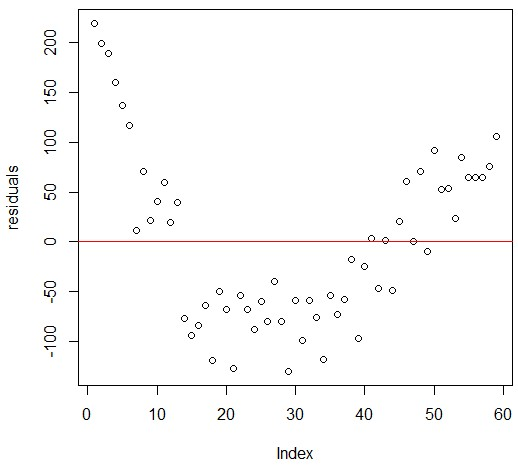
\includegraphics[width=\textwidth]{figures/res1}
		\caption{殘差分析二}
		\label{fig:res1again}
	\end{minipage}
	\begin{minipage}[b]{0.05\textwidth}
		\quad
	\end{minipage}	
	\begin{minipage}[b]{0.4\textwidth}
		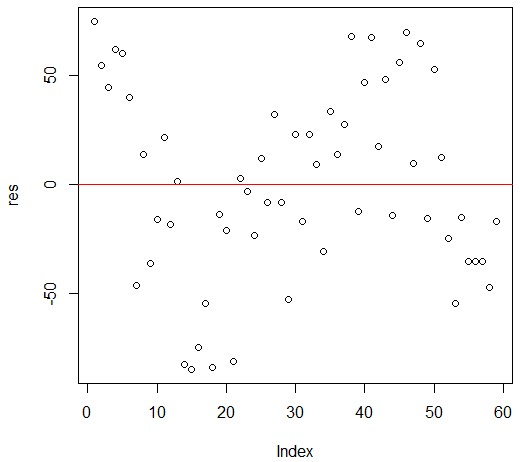
\includegraphics[width=\textwidth]{figures/res2}
		\caption{殘差分析三}
		\label{fig:res2}
	\end{minipage}
\end{figure}

\subsection{表}

正式文件的表,常常是沒有直線的,如表 \ref{tab:fre}。兩張表也可以並列,
語法跟圖併列差不多,也是利用 \verb|minipage|。在表格中,我們有時需要合併數欄或數列,
此時可以用 \verb|multirow| 與 \verb|multicolumn| 指令。

\begin{table}[hbt]
\centering
	\begin{tabular}{ccc}
	\toprule
	\multicolumn{2}{c}{年齡區間} & 次數 \\
	\midrule 
	\multirow{3}{*}{青壯年} & $[20, 30)$ & 6 \\
	& $[30, 40)$ & 18 \\
	& $[40, 50)$ & 11 \\
	\midrule
	\multirow{3}{*}{中老年} & $[50, 60)$ & 11 \\
	& $[60, 70)$ & 3 \\
	& $[70, 80)$ & 1 \\
	\bottomrule
	\end{tabular}
	\caption{這是一張表}
	\label{tab:fre}
\end{table}










\section{清單、字體與引用}

我們可以插入有編號的清單與無編號的清單:

\begin{enumerate}
\item 這是第一層。

	\begin{enumerate}
	\item 這是第二層。
	\item This is level 2. 
	\end{enumerate}
	
\item This is level 1. 

	\begin{itemize}
	\item 這是第二層。
	\item 可以任意製作巢狀清單。
	\end{itemize}

\end{enumerate}

你可以產生\textbf{粗體}或\textit{斜體};在 Texmaker 裡,熱鍵是 CTRL + B 和 CTRL + I。
This of course also applies to \textbf{English} \textit{characters}. 
有時候你會需要\texttt{typewriter font},像是要寫原始碼的時候。
另一種產生打字機字體的方法是使用 \verb|verb| 環境,兩者各有其限制,常常需要搭配使用。

你可以用 \verb|quote| 或 \verb|quotation| 引用一大段別人說的話。比如說周思齊曾經說:
\begin{quote}
我的名字,很明顯是有典故的,就是《論語》的子曰:『見賢思齊焉,見不賢而內自省也。』
看到別人的優點,要主動學習、效法,\textbf{看到不好的,要反省自己有沒有類似的錯誤。}
從唸書到打職棒,一直沒忘了姑姑為我取名字的用意,也警惕自己,在團隊生活中不可隨波逐流,
對的事情要堅持,\textbf{不對的事情也要堅持不碰就是不碰},也就是所謂的擇善固執吧。

有人問我,今年打了這麼多全壘打和打點,如果沒有拿下任何獎項會不會遺憾,我說:
\begin{center}
『人生最大的遺憾,就是沒有盡力。』
\end{center}
今年球季我沒有遺憾。
\end{quote}
\verb|quote| 和 \verb|quotation| 的效果不一樣,大家可以試試看。












\section{引用文獻}

在 \LaTeX 裡要引用文獻,最常用的是名為 BibTeX 的工具。首先,你需要製作一個副檔名為 BIB 的文獻檔,
像是附件中的 intro.bib。完成之後,你會在 TEX 檔的最後寫下如本文所寫的那兩個指令,
然後用 \citet{Cachon05} 或 \citep{Hsiao13} 來引用文獻。
\verb|citet| 是拿該篇著作當主詞時使用,\verb|citep| 則是把該篇著作放在文章結束時使用。
請注意 BIB 檔要如何編輯才能讓參考文獻的文章標題該大寫的地方大寫。

\verb|bibliographystyle| 是指定文獻格式用的,我常用的是 INFORMS 用的格式,
以 ormsv080.bst 記錄。其它常用的還有 \verb|acm|、\verb|abbrv|、
\verb|unsrt| 等等\footnote{不是每個文獻格式檔都跟 \texttt{citet} 和 \texttt{citep} 相容,
有些只相容最陽春的 \texttt{cite}。},
大家有興趣可以玩玩看,但跟我一起寫論文時還是用 ormsv080.bst 吧。
理論上中文文章應該用中文文獻格式,但實在太麻煩了,就先算了吧。
要把「References」改成「參考文獻」倒是很容易就是了。

要引用文獻時,需在編譯時多執行 BibTeX,在 Texmaker 中是按 F11。
\LaTeX 中要產生交互參照時,像是參照圖、表、方程式、文獻等等,常常需要執行同一個編譯動作連續兩次,
而執行完 BibTeX 之後還要執行 xeLaTeX(或 LaTeX 或 PDFLaTeX)才算完成,
所以當我在中文文章中有引用文獻時,我會依序按 F2、F11、F11、F2、F2、F7;
若是不用 EPS 圖形的英文文章,我會依序按 F1、F11、F11、F1、F1。










\section{結論}

我很少用 \LaTeX 打中文,畢竟還是有些麻煩,雖然比我當學生時好多了。
這一篇文章花了我差不多六個小時,請大家好好珍惜、善加利用!
一開始寫起來很慢,寫多了自然就熟了。除非時間不夠,不然還是很建議你花個一天時間,
仔細地把「cwTeX3 手冊」讀完並且跟著操作一遍,這樣就會很厲害了。
往後如果遇到不知道該下什麼指令或奇怪的錯誤,網路上十之八九都查得到,
不然就問學長姊,再不然就問我吧。

希望大家會喜歡 \LaTeX!











\bibliographystyle{ormsv080}
\bibliography{intro}

\end{document}
